\section{Introduction}
\label{sec:intro}

\begin{figure}[t]
\begin{tabular}{p{6cm}p{6cm}}
\begin{lstlisting}[basicstyle=\small]
   append$^o_{opt}$ = fun a b ab .
     ((a === Nil) /\ (ab === b)) \/
     (fresh (h t tb)
        (a === Cons(h, t)) /\
        (ab === Cons(h, tb) /\
        (append$^o_{opt}$ t b tb)))
\end{lstlisting} & \multirow{2}{*}[-3mm]{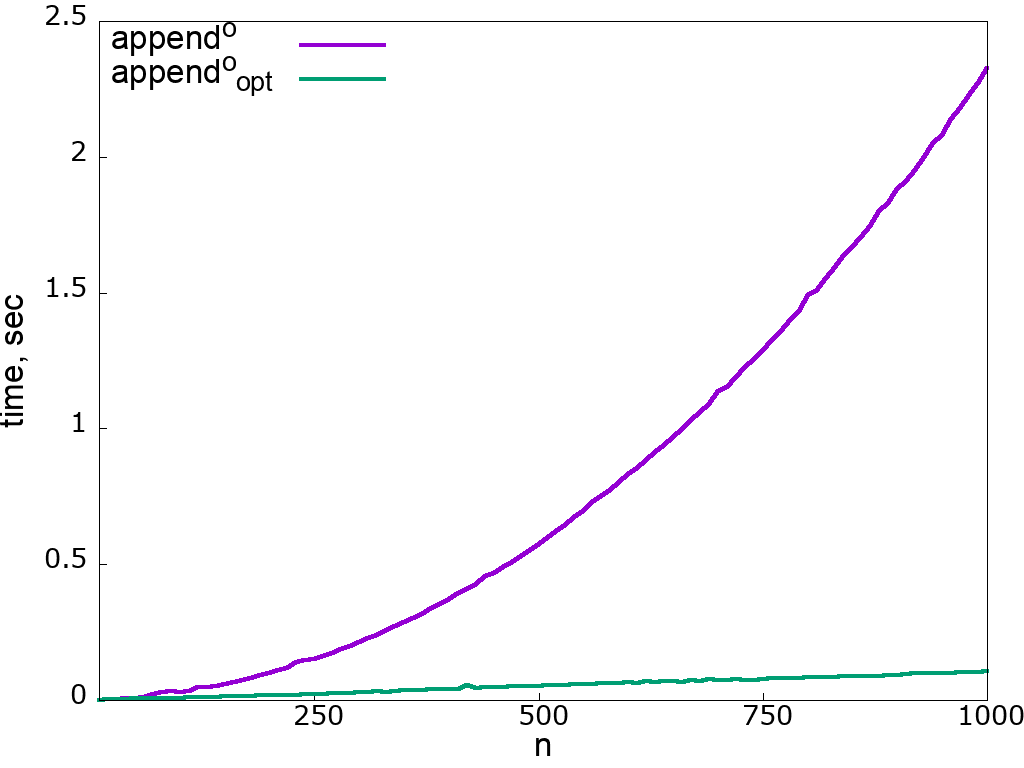
\includegraphics[width=6cm,height=5cm]{append_without_oc.png}} \\[-9mm]
\begin{lstlisting}[basicstyle=\small]
   append$^o$ = fun a b ab .
     ((a === Nil) /\ (ab === b)) \/
     (fresh (h t tb)
        (a === Cons(h, t)) /\
        (append$^o$ t b tb) /\
        (ab === Cons(h, tb)))
\end{lstlisting} &
\end{tabular}
\caption{Two implementations of list concatenation and their performance for $a = [1,\dots,n]$, $b = [1,\dots,100]$, and $ab$ left free.}
\label{fig:length_implementations}
\end{figure}

A family of embedded languages for logic and, more specifically, relational programming \mK~\cite{TRS} has demonstrated an interesting potential in various fields of 
program synthesis or declarative pogramming~\cite{SevenProblems,Quines,Matching}. A distinctive feature of \mK is \emph{interleaving search}~\cite{Transformers} which,
in particular, delivers such an important feature as completeness.

However, being a different search strategy than conventional BFS/DFS/incremental deepening, etc., interleaving search makes the conventional ways of reasoning about the complexity
of logical programs irrelevant. Moreover, some intrinsic properties of interleaving search can manifest themselves in a number of astounding and, at the first glance, unexplanable
performance effects. 

As an example, let's consider two implementations of list concatenation relation (\figureword~\ref{fig:length_implementations}, left side). The only difference between the two is
the position of the recursive call.
%A common wizdom of \mK programming prescribes putting recursive call \emph{last} in a conjunction (if possible), since otherwise multiple
%negative effects (for example, divergence) can be encountered when running a relation in a \emph{backward} direction (i.e. finding all the splits of a given list).
%What is unexpected
%is that
The evaluation of these implementations on the same problem (\figureword~\ref{fig:length_implementations}, right side) shows that the second implementation works significantly
slower,
%being run is a \emph{forward} direction as well (i.e. as a regular concatenation),
although it performs exactly the same number of unifications. As a matter of fact, these two implementations even have different \emph{asymptotic} complexity under the assumption
that occurs check is disabled.\footnote{The role of occurs check is discussed in
\sectionword~\ref{sec:evaluation}.}
A careful analysis discovers that the difference is caused not by unifications, but by the process of \emph{scheduling} goals during the search. In \mK a
lazy structure is maintained to decompose the goals into unifications, perform these unifications in a certain order, and thread the results appropriately. For the \lstinline|append$^o$|
this structure becomes linear in size, reducing the performance.

In the paper we identify two complexity measures and present a framework to derive their worst-case asymptotic estimations~--- \emph{scheduling complexity}~---
for a given goal. The goal has to fulfill a number of requirements (both syntactic and semantic), which we explicitly state in \sectionword~\ref{sec:background}. The estimations
themselves are consructed using a manual metatheory-level reasoning over a set of inequalities, which are extracted automatically using symbolic execution.
%In the paper we present a model to estimate scheduling complexity of interleaving search in \mK. We use a formal semantics which, in turn, reflects the
%behaviour of actual implementations~\cite{CertifiedSemantics}. The roadmap of our approach is as follows: we identify two complexity measures (\emph{scheduling factors}) and
%give exact and approximate recursive formulas to calculate the scheduling factors (\sectionword~\ref{sec:scheduling}); then we present an approach to
%automaticaly extract inequalities for the scheduling factors for a whole goal using symbolic execution (\sectionword~\ref{src:symbolic}). These inequalities have
%to be reformulated and solved in terms of a certain \emph{metatheory}, which, on success, provides an asymptotic bounds for the complexity of
%the goal evaluation. To be applicable, our approach puts a number of limitation on the goal being estimated as well as on the relational program as whole. We discuss
%these limitations in \sectionword~\ref{sec:discussion} as well as the contribution of scheduling in overall interleaving search complexity in \mK.
Due to space considerations, the proofs of all lemmas and theorems can be found in Appendix~\ref{sec:proofs_appendix}.


